\section{Interlocking Logic Design}
\label{sec:system-overview:interlocking-logic}

At the heart of this system lies the rule engine — a modular processor of interlocking constraints encoded in a JSON-based configuration. Its responsibilities span a variety of logical checks required to authorize safe train movements and maintain route exclusivity.

The key logic handled by the engine includes route validation, point locking, overlap reservation, and support for conditional logic. These processes are dynamically loaded from station-specific configuration files, allowing flexible deployment without recompilation. Figure~\ref{fig:interlocking-logic-overview} illustrates a conceptual overview of surface level interaction among different interlocking modules. This includes inputs from track circuits, point machines, and signal requests, and how they funnel into a layered validation process.

\begin{figure}[t]
    \centering

    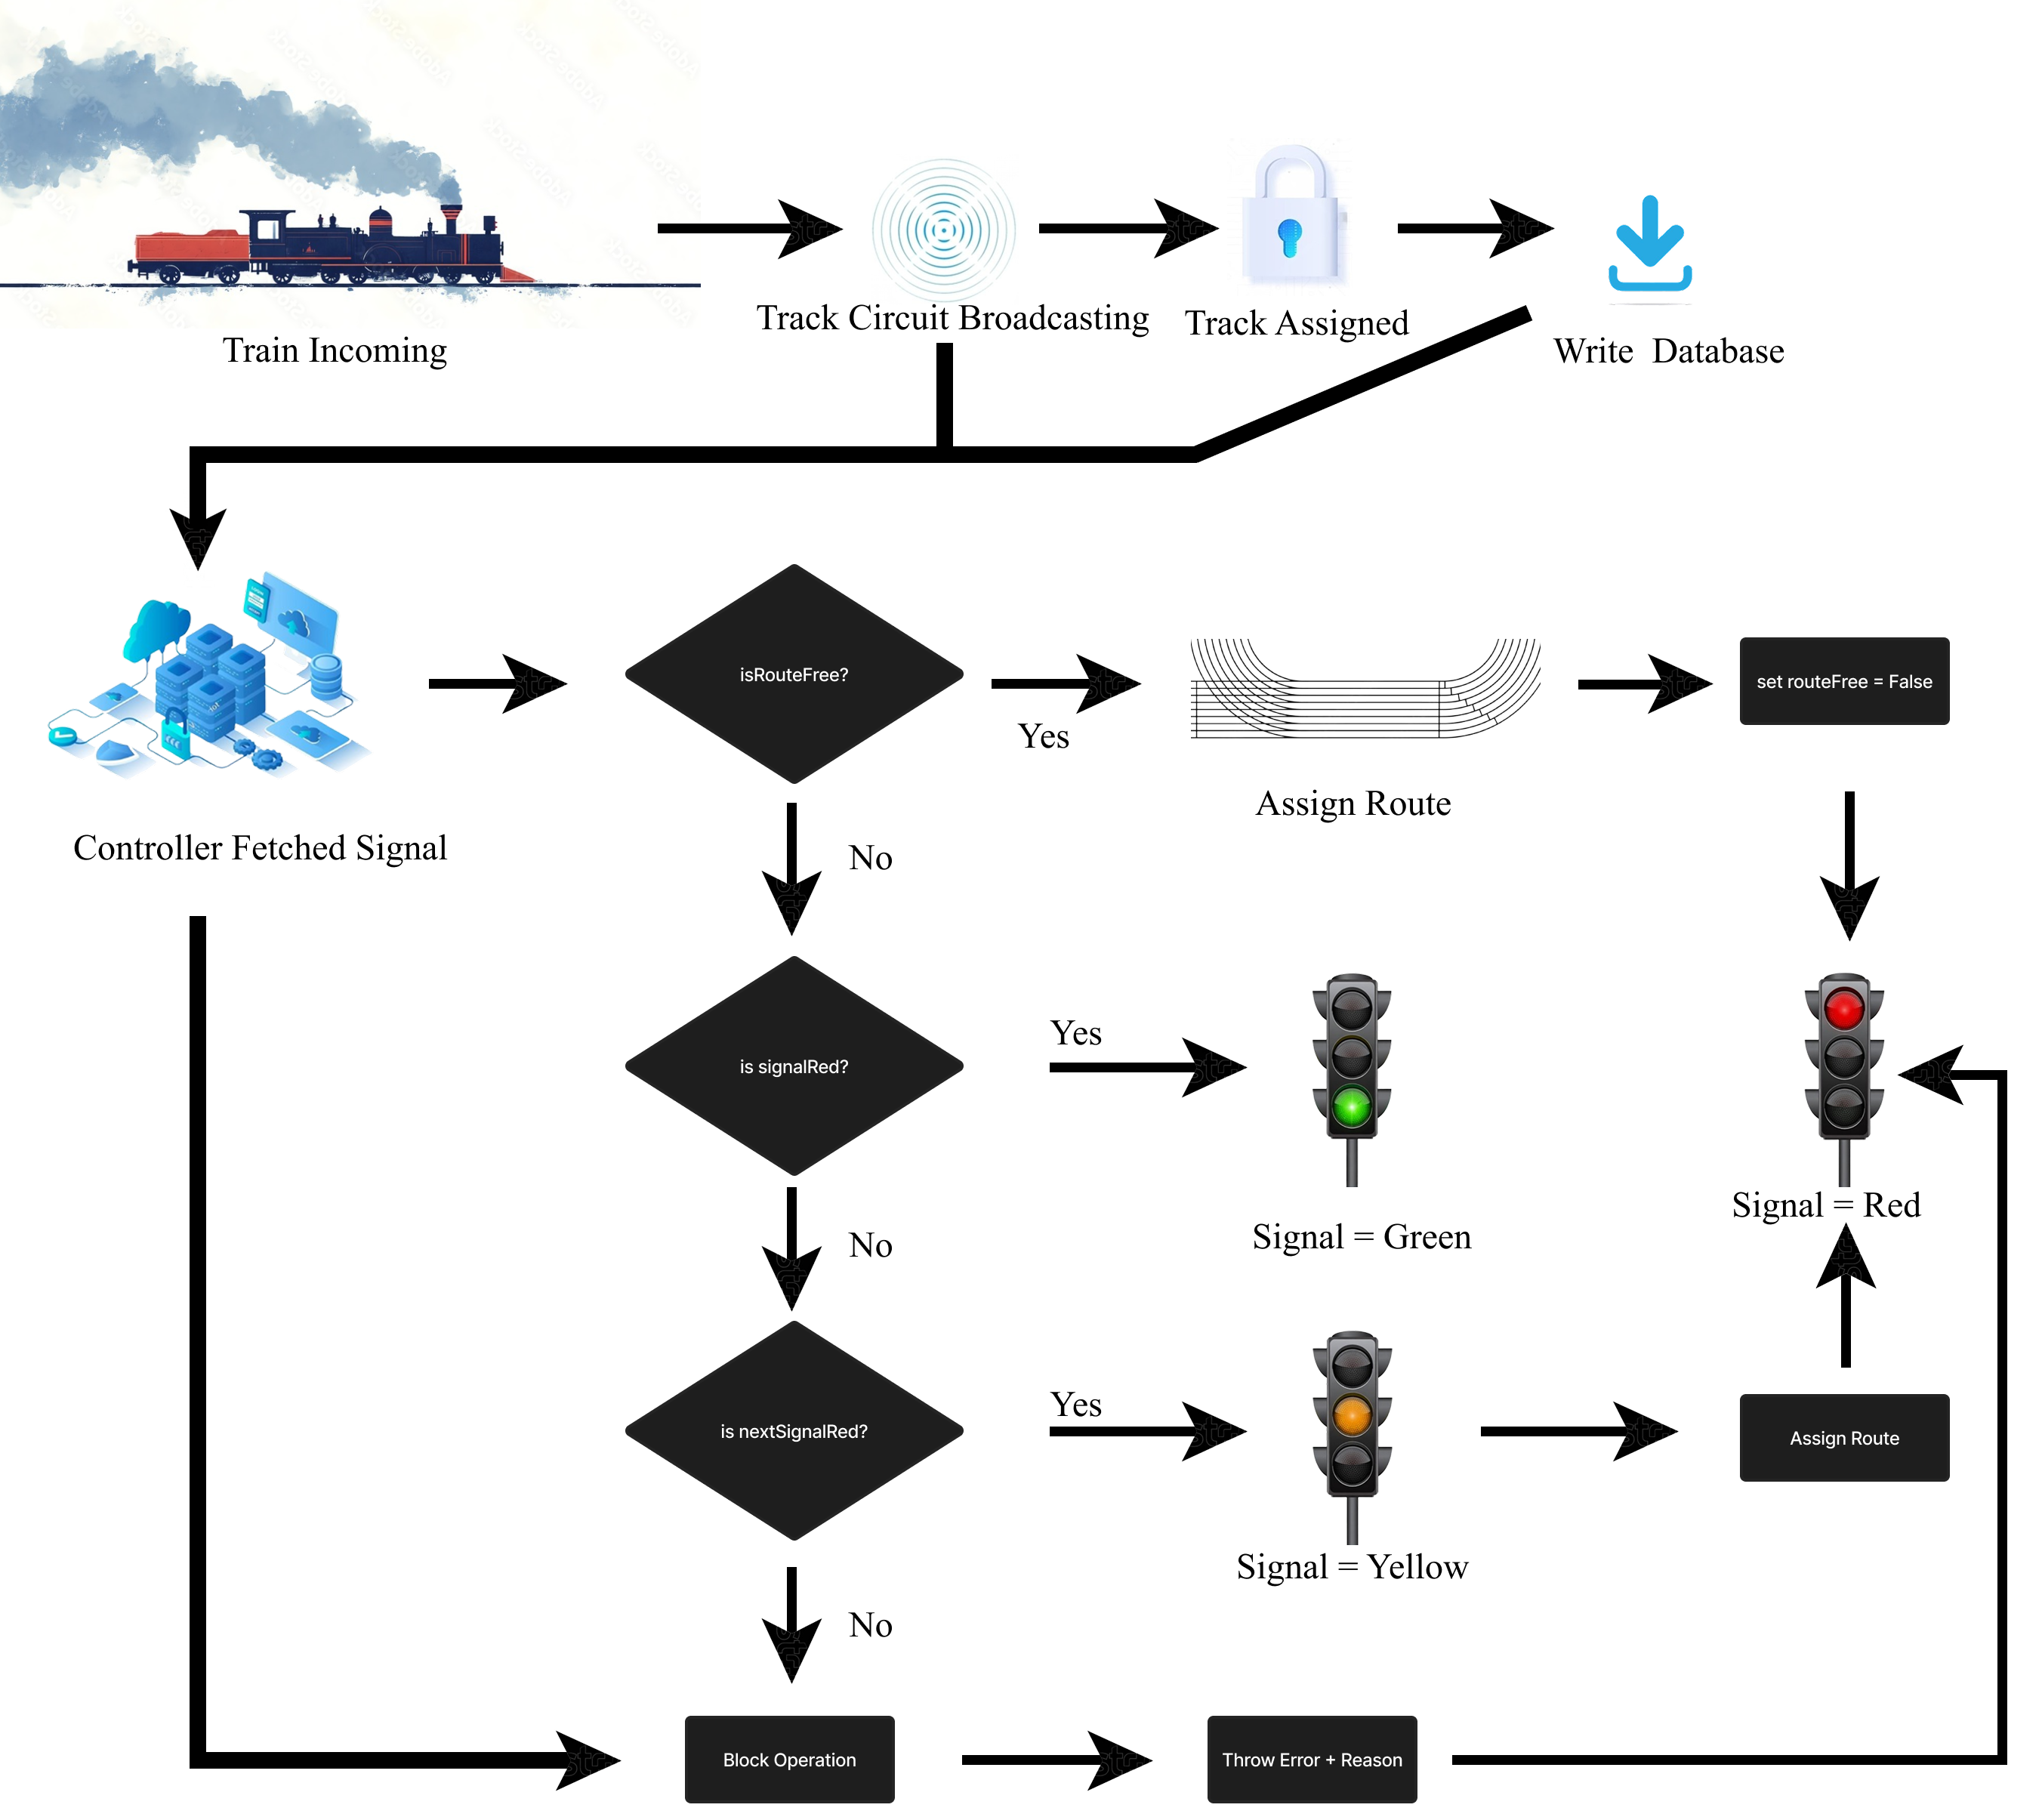
\includegraphics[width=0.85\textwidth]{images/interlocking-logic/interlocking_flow.png}

    \floatcap{Modular Interlocking Logic Flow}{Overview of validation layers including route conflict checks, point alignment, overlap safety, and conditional rule evaluation. These logic branches collectively ensure safe signal clearance.}
    
    \label{fig:interlocking-logic-overview}
\end{figure}


One of the most critical steps in this flow is route validation, where the system checks track segment occupancy, point alignment, and conflict-free paths. This process is discussed in detail in Section~\ref{sec:interlocking:route-validation} as a reference.
